
\subsection{定义}

(还记得这些定义吗?在阅读下列内容之前,请务必了解 \href{/graph/basic}{图论基础} 部分)

生成子图

生成树

最小生成树:边权和最小的生成树。

注意:只有连通图才有生成树,而对于非连通图,只能搞出生成森林。

\subsection{Kruskal 算法}

是一种常见并且好写的最小生成树算法,由 Kruskal 发明,基本思想是从小到大加入边,是个贪心算法。

\subsubsection{证明}

思路很简单,为了造出一棵最小生成树,我们从最小边权的边开始,按边权从小到大依次加入,如果某次加边产生了环,就扔掉这条边,直到加入了 $n-1$ 条边,即形成了一棵树。

证明:使用归纳法,证明任何时候 K 算法选择的边集都被某棵 MST 所包含。

基础:对于算法刚开始时,显然成立(最小生成树存在)。

归纳:假设某时刻成立,当前边集为 $F$,令 $T$ 为这棵 MST,考虑下一条加入的边 $e$。

如果 $e$ 属于 $T$,那么成立。

否则,$T+e$ 一定存在一个环,考虑这个环上不属于 $F$ 的另一条边 $f$(一定只有一条)。

首先,$f$ 的权值一定不会比 $e$ 小,不然 $f$ 会在 $e$ 之前被选取。

然后,$f$ 的权值一定不会比 $e$ 大,不然 $T+e-f$ 就是一棵比 $T$ 还优的生成树了。

所以,$T+e-f$ 包含了 $F$,并且也是一棵最小生成树,归纳成立。

\subsubsection{实现}

算法虽简单,但需要相应的数据结构来支持……

具体来说,维护一个森林,查询两个结点是否在同一棵树中,连接两棵树。

抽象一点地说,维护一堆 \textbf{集合},查询两个元素是否属于同一集合,合并两个集合。

我们先啥都不管,假设已经实现了这个数据结构……

(伪代码)

\vskip 0.2 in
\texttt{
for (edge(u, v, len) in sorted(edges)) {\\	a = find_set(u), b = find_set(v);\\	if (a != b) merge(a, b);\\}}
\vskip 0.2 in

\texttt{find_set} 调用 $O(m)$ 次,merge 调用 $O(n)$ 次。

排序的复杂度为 $O(m \log m)$,或 $O(m)$(假设能基数排序)。

那么让我们模拟一下:

先上数据:

\vskip 0.2 in
\texttt{
4 5\\1 2 2\\1 3 2\\1 4 3\\2 3 4\\3 4 3}
\vskip 0.2 in

图是这样的:

\begin{figure}[h]
\centering
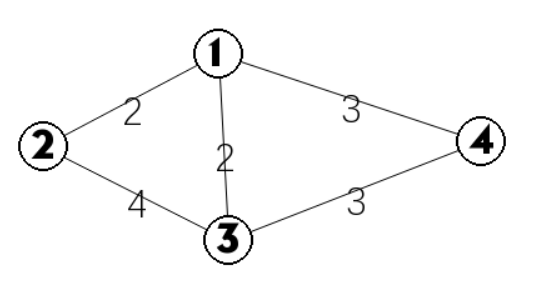
\includegraphics[width=0.5\textwidth]{images/mst1.png} 

\end{figure}

我们用 $F$ 表示并查集, $E$ 表示排序后的结构体,下面是初始的状态:

$F$:

\begin{tabular}{rrrrr}
\hline
编号& 1& 2& 3& 4\\祖宗& 1& 2& 3& 4\\\hline
\end{tabular}

$E$:

\begin{tabular}{rrrrrr}
\hline
编号& 1& 2& 3& 4& 5\\start& 1& 1& 1& 3& 2\\to& 2& 3& 4& 4& 3\\cost& 2& 2& 3& 3& 4\\\hline
\end{tabular}

首先我们发现 1,2 是最小的,于是我们在 1 与 2 建了一条边,由于这是第一次嘛,肯定不会出现环了,并且将 1 和 2 加入一个集合:

\begin{figure}[h]
\centering
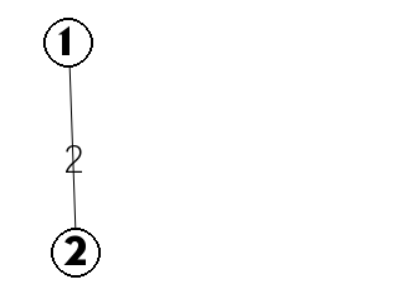
\includegraphics[width=0.5\textwidth]{images/mst2.png} 

\end{figure}

$F$:

\begin{tabular}{rrrrr}
\hline
编号& 1& 2& 3& 4\\祖宗& 1& 1& 3& 4\\\hline
\end{tabular}

接着发现 1,3,判断 3 和 1 的是不是在一个集合?发现不是,于是将 3 加进去,并且标记 3 归属1。

\begin{figure}[h]
\centering
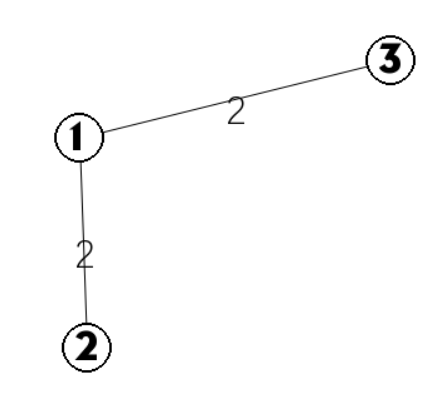
\includegraphics[width=0.5\textwidth]{images/mst3.png} 

\end{figure}

$F$:

\begin{tabular}{rrrrr}
\hline
编号& 1& 2& 3& 4\\祖宗& 1& 1& 1& 4\\\hline
\end{tabular}

发现 1,4,同时 1 和 4 不在一个集合,于是将 4 加进去,标记 4 也归属 1。

\begin{figure}[h]
\centering
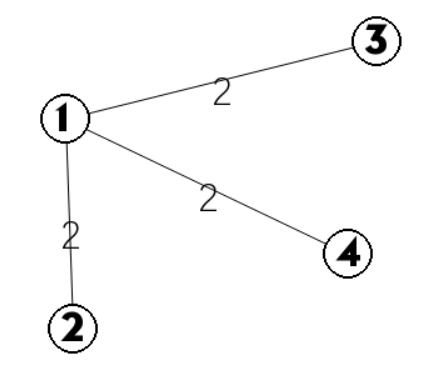
\includegraphics[width=0.5\textwidth]{images/mst4.png} 

\end{figure}

\begin{tabular}{rrrrr}
\hline
编号& 1& 2& 3& 4\\祖宗& 1& 1& 1& 1\\\hline
\end{tabular}

此时,边数为点数 $-1$,整个最小生成树完成了,代价是 $2+2+3=7$。

\subsubsection{“集合” 数据结构的一种实现}

只要支持两个接口:find\_set 和 merge。

我们先考虑暴力,直接维护每个元素属于哪个集合,以及每个集合有哪些元素。

find\_set:$O(1)$

merge:$O(n)$,需要将一个集合中的所有元素移到另一个集合中。

于是考虑如何优化 merge。

一个简单的思路是,将较小的集合中所有元素移到较大的集合中。

复杂度是 $O(较小集合的大小)$。

那么总时间复杂度是多少呢?

我们换一个角度分析,考虑每个元素对每次合并操作的贡献。

很显然,一个元素所在的集合大小,在作为较小集合被合并一次之后,至少增加一倍。

所以一个元素所在的集合,最多有 $\log n$ 次,作为较小集合被合并。

一共$n$个元素,所以总时间复杂度为 $O(n \log n + m)$。

这种做法或者思想,叫「启发式合并」。

总之我们得到了 $O(n \log n + m \log m)$ 的 Kruskal 算法。

\subsection{Prim 算法}

是另一种常见并且好写的最小生成树算法。

基本思想是从一个结点开始,不断加点(而不是 Kruskal 算法的加边)。

\subsubsection{证明}

从任意一个结点开始,将结点分成两类:已加入的,未加入的。

每次从未加入的结点中,找一个与已加入的结点之间边权最小值最小的结点。

然后将这个结点加入,并连上那条边权最小的边。

重复 $n-1$ 次即可。

证明:还是说明在每一步,都存在一棵最小生成树包含已选边集。

基础:只有一个结点的时候,显然成立。

归纳:如果某一步成立,当前边集为 $F$,属于 $T$ 这棵 MST,接下来要加入边 $e$。

如果 $e$ 属于 $T$,那么成立。

否则考虑 $T+e$ 中环上另一条可以加入当前边集的边 $f$。

首先,$f$ 的权值一定不小于 $e$ 的权值,否则就会选择 $f$ 而不是 $e$ 了。

然后,$f$ 的权值一定不大于 $e$ 的权值,否则 $T+e-f$ 就是一棵更小的生成树了。

因此,$e$ 和 $f$ 的权值相等,$T+e-f$ 也是一棵最小生成树,且包含了 $F$。

\subsubsection{实现}

也是需要一些数据结构来支持。

具体来说,每次要选择距离最小的一个结点,以及用新的边更新其他结点的距离。

等等,这很像 Dijkstra 算法……

其实跟 Dijkstra 算法一样,只要一个堆来维护距离即可。

暴力:$O(n^2+m)$。

二叉堆:$O((n+m) \log n)$。

Fib 堆:$O(n \log n + m)$。

(伪代码)

\vskip 0.2 in
\texttt{
H = new heap();\\for (i = 1; i <= n; i++) H.insert(i, inf);\\H.decrease_key(1, 0);\\for (i = 1; i <= n; i++) {\\	u = H.delete_min();\\	for each edge(u, v, len) {\\		H.decrease_key(v, len);\\	}\\}}
\vskip 0.2 in

注意:上述代码只是实现了 Prim 算法主体,如果要输出方案还需要记录额外的信息。

注意:在遍历边表 \texttt{(u, v)} 时,如果 v 已经被 delete,就无需 decrease key。

\subsection{最小生成树小结}

我们介绍了两种最小生成树的算法,各有特点。

然后我们来考虑这样一些问题。

一张图的最小生成树不一定是唯一的。

什么时候一定唯一?

考虑 Kruskal 算法,当每条边权都不一样时,一开始的排序只有一种方案,就一定唯一了。

那什么时候一定不唯一?

Kruskal 算法中的「集合」,能否进一步优化?

\subsection{最小生成树题目}

\href{https://www.lydsy.com/JudgeOnline/problem.php?id=2429}{\textbackslash{}[HAOI2006\textbackslash{}] 聪明的猴子}

\href{https://www.lydsy.com/JudgeOnline/problem.php?id=1083}{\textbackslash{}[SCOI2005\textbackslash{}] 繁忙的都市}

\subsection{最小生成树的唯一性}

考虑最小生成树的唯一性。如果一条边\textbf{不在最小生成树的边集中},并且可以替换与其\textbf{权值相同、并且在最小生成树边集}的另一条边。那么,这个最小生成树就是不唯一的。

对于 Kruskal 算法,只要计算为当前权值的边可以放几条,实际放了几条,如果这两个值不一样,那么就说明这几条边与之前的边产生了一个环(这个环中至少有两条当前权值的边,否则根据并查集,这条边是不能放的),即最小生成树不唯一。

寻找权值与当前边相同的边,我们只需要记录头尾指针,用单调队列即可在$O(\alpha(m))$(m 为边数)的时间复杂度里优秀解决这个问题(基本与原算法时间相同)。

\begin{NOTE}{ 例题:[POJ 1679](http://poj.org/problem?id=1679)}{}

\end{NOTE}


\vskip 0.2 in
\texttt{
```cpp\\#include <algorithm>\\#include <cstdio>\\using namespace std;\\struct tree\\{\\  int x,y,z;\\};\\int f[100001];\\tree a[100001];\\int cmp(const tree a,const tree b)\\{\\  return a.z<b.z;\\}\\int find(int x)\\{\\  if (f[x]==x) return x;\\  f[x]=find(f[x]);\\  return f[x];\\}\\int main()\\{\\  int t;\\  scanf("%d",&t);\\  while (t--)\\  {\\    int n,m;\\    scanf("%d%d",&n,&m);\\    for (int i=1;i<=n;i++) f[i]=i;\\    for (int i=1;i<=m;i++)\\      scanf("%d%d%d",&a[i].x,&a[i].y,&a[i].z);\\    sort(a+1,a+m+1,cmp);\\    int num=0;\\    int ans=0;\\    int tail=0;\\    int sum1=0;\\    int sum2=0;\\    int flag=1;\\    for (int i=1;i<=m+1;i++)\\    {\\      if (i>tail)\\      {\\        if (sum1!=sum2)\\        {		\\          flag=0;break;\\        }\\        sum1=0;\\        for (int j=i;j<=m+1;j++)\\        {\\          if (a[j].z!=a[i].z) \\          {\\            tail=j-1;break;\\          }\\          if (find(a[j].x)!=find(a[j].y)) ++sum1;\\        }\\        sum2=0;\\      }\\      if (i>m) break;\\      int x=find(a[i].x);\\      int y=find(a[i].y);\\      if (x!=y&&num!=n-1)\\      {\\        sum2++;\\        num++;\\        f[x]=f[y];\\        ans+=a[i].z;\\      }\\    }\\    if (flag) printf("%d\n",ans);\\    else printf("Not Unique!\n");\\  }\\  return 0;\\}\\```}
\vskip 0.2 in

\subsection{次小生成树}

\subsection{第 k 小生成树}
